\section{Shared caching layer between the micro-frontends}\label{section:applied-methods:shared-caching-layer}

\noindent With the learnings from the previous section \ref{section:applied-methods:communication-shell-remote} on how to communicate between different micro-frontends, a shared caching layer should be developed. This section describes how the shared caching layer was implemented and how it can be used inside the application. The structure of the shared caching layer should look like in the figure \ref{fig:applied-methods:structure-shared-caching-layer}. The micro-frontends have their instance of the Apollo Client, but they should all use the same instance of the in-memory cache. Therefore, each application can provide configuration for the Apollo Client, but they all use the same cache instance. The in-memory cache stores the results of the GraphQL queries, and if the micro-frontends need to fetch the same data, they can use the data from the cache instead of fetching it from the server again. The approach reduces the number of network requests and, therefore, the amount of data that has to be transferred over the network. 

\ifshowImages
  \begin{figure}[H]
  \centering
  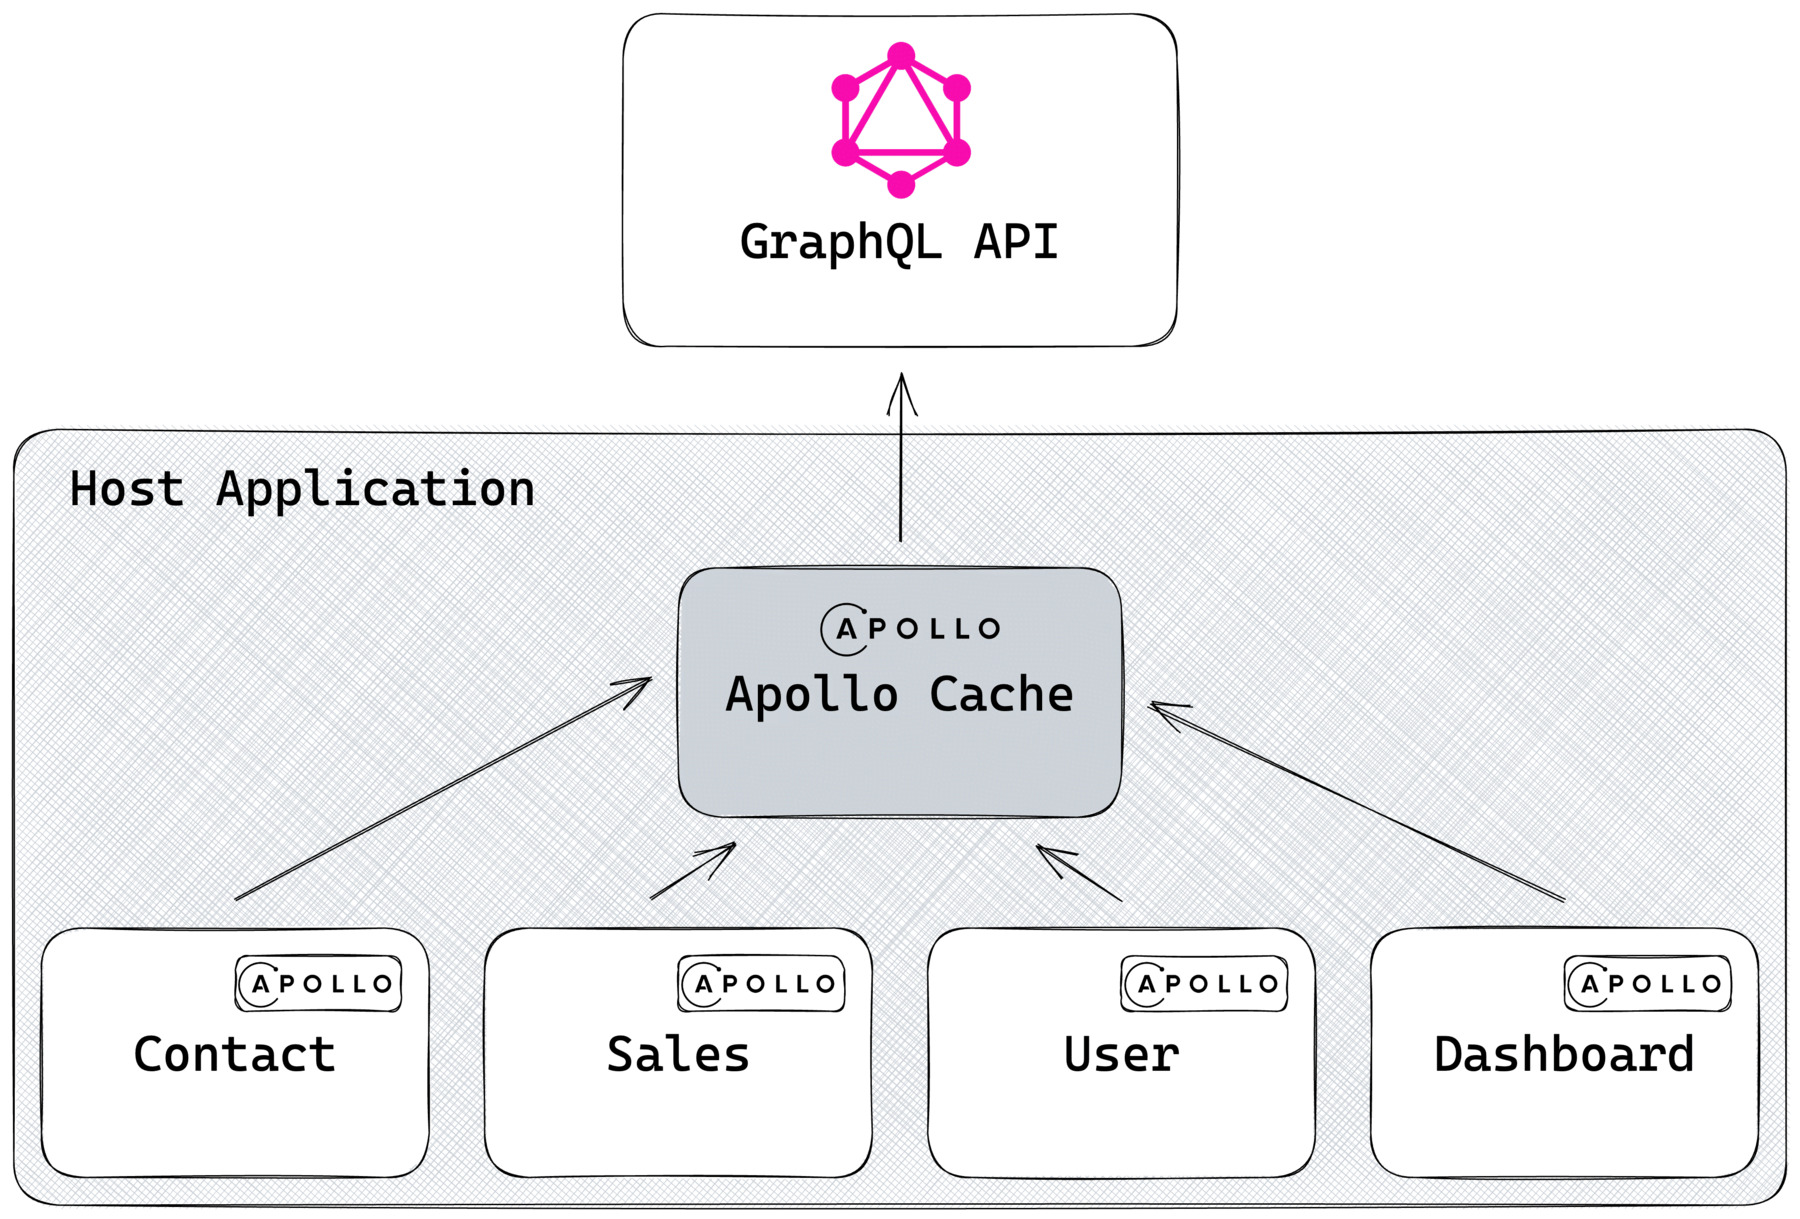
\includegraphics[width=0.8\linewidth]{images/applied-methods/shared-caching-layer/shared-caching-layer.jpg}
  \caption{The structure of the shared caching layer.}\label{fig:applied-methods:structure-shared-caching-layer}
  \end{figure}
\fi

\noindent The application shell should provide the instance of the GraphQL cache. The listing \ref{code:applied-methods:creating-the-apollo-client} shows how the Apollo Client is created for an application with default settings. The \textbf{cache} property is important, as it receives the instance of the in-memory cache. Therefore, the cache instance can be created elsewhere and passed to the Apollo Client. 
\ifshowListings
\begin{listing}[H]
\begin{minted}{typescript}
@NgModule({
  imports: [ApolloModule],
  providers: [{
    provide: APOLLO_OPTIONS,
    useFactory: (httpLink: HttpLink) => ({
      cache: new InMemoryCache(),
      link: httpLink.create({ uri: 'http://localhost:3000' }),
    }),
    deps: [HttpLink],
  }]
})
class AppModule {}
\end{minted}
\caption{Creating an instance of the Apollo Client.}\label{code:applied-methods:creating-the-apollo-client}
\end{listing}
\fi

\noindent The idea is to define the cache instance inside the application shell and provide it to the remote applications. The instance of the in-memory cache should be provided through an injection token, just like the injection token from the section \ref{section:applied-methods:communication-shell-remote}, that specifies whether the application shell consumes the applications or runs in standalone mode. The injection token can be provided by the application shell and injected by the remote modules of the micro-frontends. Moreover, the application can provide the token when it runs in standalone mode. The provider can be implemented by providing the instance of the cache through an injection token called \texttt{GRAPHQL\_CLIENT\_CACHE}, as shown in the listing \ref{code:applied-methods:graphql-client-cache-provider}.

\ifshowListings
\begin{listing}[H]
\begin{minted}{typescript}
@NgModule({
  providers: [
    { provide: GRAPHQL_CLIENT_CACHE, useValue: new InMemoryCache() }
  ]
})
class HostCoreModule {}
\end{minted}
\caption{Provide the instance of the in-memory cache to \ac{DI}.}\label{code:applied-methods:graphql-client-cache-provider}
\end{listing}
\fi


\ifshowListings
\begin{listing}[H]
\begin{minted}{typescript}
@NgModule({
  imports: [ApolloModule],
  providers: [{
    provide: APOLLO_OPTIONS,
    useFactory(httpLink: HttpLink, cache: InMemoryCache) {
      const link = httpLink.create({uri: 'http://localhost:3000'});
      return { cache, link };
    },
    deps: [HttpLink, GRAPHQL_CLIENT_CACHE],
  }]
})
class ContactRemoteModule {}
\end{minted}
\caption{Using the shared in-memory cache instance.}\label{code:applied-methods:creating-the-apollo-client-with-a-shared-cache}
\end{listing}
\fi

\noindent The micro-frontend prototype architecture provides abstractions to create the necessary configuration for the Apollo Client more easily. Listing \ref{code:applied-methods:graphql-client-creation} shows the abstraction. The method provides the importing module with an instance of the Apollo Client. The method takes one required parameter that specifies a unique name for the client. The client's name is used to identify all active Apollo Clients inside the architecture. The module encapsulates the steps to create an Apollo Client, as shown in the listing \ref{code:applied-methods:creating-the-apollo-client-with-a-shared-cache}. The module should be used in every module exposed through Module Federation. If the remote module is then used inside the application shell, it has its separate Apollo Client. That makes the independent development of the micro-frontends easier because the GraphQL client's settings will be the same, independent of the environment where it is running. For example, a problem would be if the application shell provides the Apollo Client and the contact micro-frontend injects that instance with \ac{DI}. The contact team might configure the Apollo Client differently in the contact application, and the code might not work as expected inside the application because the configuration is different.

\ifshowListings
  \begin{listing}[H]
    \begin{minted}{typescript}
@NgModule({
  imports: [ GraphQLClientOptionsModule.withConfig('contact-remote') ]
})
class ContactRemoteCoreModule {}
    \end{minted}
  \caption{Instantiating Apollo Client for the module.}\label{code:applied-methods:graphql-client-creation}
  \end{listing}
\fi

\noindent The function creates a new Apollo Client instance with specified default settings. The \ac{URL} of the GraphQL \ac{API} is taken from the storage service. By default, it tries to inject the \texttt{GRAPHQL\_CLIENT\_CACHE}, to use the shared. If it cannot be injected, it creates a separate instance for the client. An injection token named \texttt{GRAPHQL\_CLIENT\_OPTIONS\_CONFIG} can be used to specify further options for creating the Apollo Client. The injection token's usage and default options are shown inside listing \ref{code:applied-methods:graphql-client-extra-configuration-options}. The injection token must be specified inside the same module where the \texttt{GraphQLClientOptionsModule} was defined.

\ifshowListings
\begin{listing}[H]
\begin{minted}{typescript}
@NgModule({
  providers: [{
    provide: GRAPHQL_CLIENT_OPTIONS_CONFIG,
    useValue: {
      shareCache: true,
      persistCache: false,
      useTypePolicies: true,
      typePolicies: CONTACT_TYPE_POLICIES,
    },
  }]
})
class ContactRemoteCoreModule {}
\end{minted}
\caption{Additional options for creating the Apollo Client instance.}\label{code:applied-methods:graphql-client-extra-configuration-options}
\end{listing}
\fi

\noindent The options include \texttt{shareCache}, \texttt{persistCache}, \texttt{useTypePolicies} and \texttt{typePolicies}. \texttt{shareCache} is used to specify if the Apollo Client should use the in-memory cache instance from \texttt{GRAPHQL\_CLIENT\_CACHE} or if it should create a new instance, specifically for this module. The \texttt{persistCache} option is \texttt{false} by default. It stores the contents of the in-memory cache inside the \texttt{localStorage}. This feature provided by the Apollo Client allows the page to be rendered faster initially because the data from the \texttt{localStorage} is inserted into the cache when the page loads. The options \texttt{useTypePolicies} and \texttt{typePolicies} belong together and must be specified. The property \texttt{useTypePolicies} specifies whether the \texttt{typePolicies} should be used or not. Type policies allow Apollo Client to customize the read and write operations for the cache. They are explained in more detail in section \ref{subsubsection:background:graphql:apollo-server-client:type-policies}. Every micro-frontend has a separate Apollo Client, with a shared cache, therefore, the type policies cannot be registered directly when creating the \texttt{InMemoryCache}. The option \texttt{typePolicies} is identical to the parameter \texttt{typePolicies} of the \texttt{InMemoryCache} constructor. Specifying the option when providing the \texttt{GRAPHQL\_CLIENT\_OPTIONS\_CONFIG} allows the micro-frontend to specify additional type policies for the cache. Part of the code of the abstraction to create the Apollo Client is shown in listing \ref{code:applied-methods:adding-extra-type-policies}. First, the instance of the cache is injected. If the cache cannot be injected, it means that the Apollo Client should create a new instance of the cache. The \texttt{typePolicies} are added to the cache if the options \texttt{typePolicies} and \texttt{useTypePolicies} are both \texttt{true}.

\ifshowListings
\begin{listing}[H]
\begin{minted}{typescript}
const cache = inject(GRAPHQL_CLIENT_CACHE, { optional: true });
const { shareCache, useTypePolicies, typePolicies } = graphQLClientOptions;

const cacheInstance = shareCache ? cache : new InMemoryCache();

if (typePolicies && useTypePolicies)
  clientCache.policies.addTypePolicies(typePolicies);
\end{minted}
\caption{Adding type policies to the cache.}\label{code:applied-methods:adding-extra-type-policies}
\end{listing}
\fi

\noindent The prototype architecture follows the approach that each micro-frontend has a separate GraphQL client and a shared cache. That allows for the most flexibility as each micro frontend can configure the GraphQL client individually.